\documentclass[12pt,a4paper]{book}
\usepackage{lmodern}
\usepackage{amssymb,amsmath}
\usepackage{ifxetex,ifluatex}
\usepackage{fixltx2e} % provides \textsubscript
\ifnum 0\ifxetex 1\fi\ifluatex 1\fi=0 % if pdftex
  \usepackage[T1]{fontenc}
  \usepackage[utf8]{inputenc}
\else % if luatex or xelatex
  \ifxetex
    \usepackage{mathspec}
  \else
    \usepackage{fontspec}
  \fi
  \defaultfontfeatures{Ligatures=TeX,Scale=MatchLowercase}
\fi
% use upquote if available, for straight quotes in verbatim environments
\IfFileExists{upquote.sty}{\usepackage{upquote}}{}
% use microtype if available
\IfFileExists{microtype.sty}{%
\usepackage{microtype}
\UseMicrotypeSet[protrusion]{basicmath} % disable protrusion for tt fonts
}{}
\usepackage[margin=2cm]{geometry}
\usepackage{hyperref}
\PassOptionsToPackage{usenames,dvipsnames}{color} % color is loaded by hyperref
\hypersetup{unicode=true,
            pdftitle={Notes on a design of a simple spatial sampling method (S3M) for assessing coverage of health and nutrition programmes in Liberia},
            pdfauthor={Valid International},
            colorlinks=true,
            linkcolor=Maroon,
            citecolor=Blue,
            urlcolor=Blue,
            breaklinks=true}
\urlstyle{same}  % don't use monospace font for urls
\usepackage{natbib}
\bibliographystyle{apalike}
\usepackage{longtable,booktabs}
\usepackage{graphicx,grffile}
\makeatletter
\def\maxwidth{\ifdim\Gin@nat@width>\linewidth\linewidth\else\Gin@nat@width\fi}
\def\maxheight{\ifdim\Gin@nat@height>\textheight\textheight\else\Gin@nat@height\fi}
\makeatother
% Scale images if necessary, so that they will not overflow the page
% margins by default, and it is still possible to overwrite the defaults
% using explicit options in \includegraphics[width, height, ...]{}
\setkeys{Gin}{width=\maxwidth,height=\maxheight,keepaspectratio}
\IfFileExists{parskip.sty}{%
\usepackage{parskip}
}{% else
\setlength{\parindent}{0pt}
\setlength{\parskip}{6pt plus 2pt minus 1pt}
}
\setlength{\emergencystretch}{3em}  % prevent overfull lines
\providecommand{\tightlist}{%
  \setlength{\itemsep}{0pt}\setlength{\parskip}{0pt}}
\setcounter{secnumdepth}{5}
% Redefines (sub)paragraphs to behave more like sections
\ifx\paragraph\undefined\else
\let\oldparagraph\paragraph
\renewcommand{\paragraph}[1]{\oldparagraph{#1}\mbox{}}
\fi
\ifx\subparagraph\undefined\else
\let\oldsubparagraph\subparagraph
\renewcommand{\subparagraph}[1]{\oldsubparagraph{#1}\mbox{}}
\fi

%%% Use protect on footnotes to avoid problems with footnotes in titles
\let\rmarkdownfootnote\footnote%
\def\footnote{\protect\rmarkdownfootnote}

%%% Change title format to be more compact
\usepackage{titling}

% Create subtitle command for use in maketitle
\newcommand{\subtitle}[1]{
  \posttitle{
    \begin{center}\large#1\end{center}
    }
}

\setlength{\droptitle}{-2em}

  \title{Notes on a design of a simple spatial sampling method (S3M) for
assessing coverage of health and nutrition programmes in Liberia}
    \pretitle{\vspace{\droptitle}\centering\huge}
  \posttitle{\par}
    \author{Valid International}
    \preauthor{\centering\large\emph}
  \postauthor{\par}
      \predate{\centering\large\emph}
  \postdate{\par}
    \date{2018-07-30}

\usepackage{booktabs}
\usepackage{color}
\usepackage{tcolorbox}
\usepackage{float}
\usepackage{setspace}

\onehalfspacing

\graphicspath{ {icons/} }

\newenvironment{rmdremind}
  {\begin{tcolorbox}[width=\textwidth, 
                     colback = {white}, 
                     title = {\textbf{Remember}}, 
                     colbacktitle = lightgray,
                     coltitle = black]
  \begin{includegraphics}[scale = 1]{remind.png}
  \begin{itemize}}
  {\end{itemize}
  \end{includegraphics}
  \end{tcolorbox}}

\newenvironment{rmdnote}
  {\begin{tcolorbox}[width=\textwidth, 
                     colback = {white}, 
                     title = {\textbf{Note}}, 
                     colbacktitle = lightgray,
                     coltitle = black]
  \begin{includegraphics}[scale = 1]{pencil.png}}
  {\end{includegraphics}
  \end{tcolorbox}}
  
\newenvironment{rmdcalc}
  {\begin{tcolorbox}[width=\textwidth, 
                     colback = {white}, 
                     title = {\textbf{Calculations}}, 
                     colbacktitle = lightgray,
                     coltitle = black]
  \begin{includegraphics}[scale = 2]{pencil.png}}
  {\end{includegraphics}
  \end{tcolorbox}}
  
\newenvironment{rmdexercise}
  {\begin{tcolorbox}[width=\textwidth, 
                     colback = {white}, 
                     title = {\textbf{Exercise}}, 
                     colbacktitle = lightgray,
                     coltitle = black]
  \begin{includegraphics}[scale = 1]{exercise.png}}
  {\end{includegraphics}
  \end{tcolorbox}}
  
\newenvironment{rmdbox}
  {\begin{tcolorbox}[width=\textwidth, 
                     colback = {white}, 
                     title = {\textbf{Exercise}}, 
                     colbacktitle = lightgray,
                     coltitle = black]
  \begin{includegraphics}[scale = 1]{pencil.png}}
  {\end{includegraphics}
  \end{tcolorbox}}
  
\newenvironment{rmdinfo}
  {\begin{tcolorbox}[width=\textwidth, 
                     colback = {white}, 
                     title = {\textbf{Info}}, 
                     colbacktitle = lightgray,
                     coltitle = black]
  \begin{includegraphics}[scale = 1]{info.png}}
  {\end{includegraphics}
  \end{tcolorbox}}  
  
\newenvironment{rmdwarning}
  {\begin{tcolorbox}[width=\textwidth, 
                     colback = {white}, 
                     title = {\textbf{Warning}}, 
                     colbacktitle = lightgray,
                     coltitle = black]
  \begin{includegraphics}[scale = 1]{warning.png}}
  {\end{includegraphics}
  \end{tcolorbox}}

\newenvironment{rmdcaution}
  {\begin{tcolorbox}[width=\textwidth, 
                     colback = {white}, 
                     title = {\textbf{Caution}}, 
                     colbacktitle = lightgray,
                     coltitle = black]
  \begin{includegraphics}[scale = 1]{warning.png}}
  {\end{includegraphics}
  \end{tcolorbox}}

\newenvironment{rmddownload}
  {\begin{tcolorbox}[width=\textwidth, 
                     colback = {white}, 
                     title = {\textbf{Download}}, 
                     colbacktitle = lightgray,
                     coltitle = black]
  \begin{includegraphics}[scale = 1]{download.png}}
  {\end{includegraphics}
  \end{tcolorbox}}

\usepackage{amsthm}
\newtheorem{theorem}{Theorem}[chapter]
\newtheorem{lemma}{Lemma}[chapter]
\theoremstyle{definition}
\newtheorem{definition}{Definition}[chapter]
\newtheorem{corollary}{Corollary}[chapter]
\newtheorem{proposition}{Proposition}[chapter]
\theoremstyle{definition}
\newtheorem{example}{Example}[chapter]
\theoremstyle{definition}
\newtheorem{exercise}{Exercise}[chapter]
\theoremstyle{remark}
\newtheorem*{remark}{Remark}
\newtheorem*{solution}{Solution}
\let\BeginKnitrBlock\begin \let\EndKnitrBlock\end
\begin{document}
\maketitle

{
\hypersetup{linkcolor=black}
\setcounter{tocdepth}{1}
\tableofcontents
}
\hypertarget{simple-spatial-sampling-method-s3m}{%
\chapter*{Simple Spatial Sampling Method
(S3M)}\label{simple-spatial-sampling-method-s3m}}
\addcontentsline{toc}{chapter}{Simple Spatial Sampling Method (S3M)}

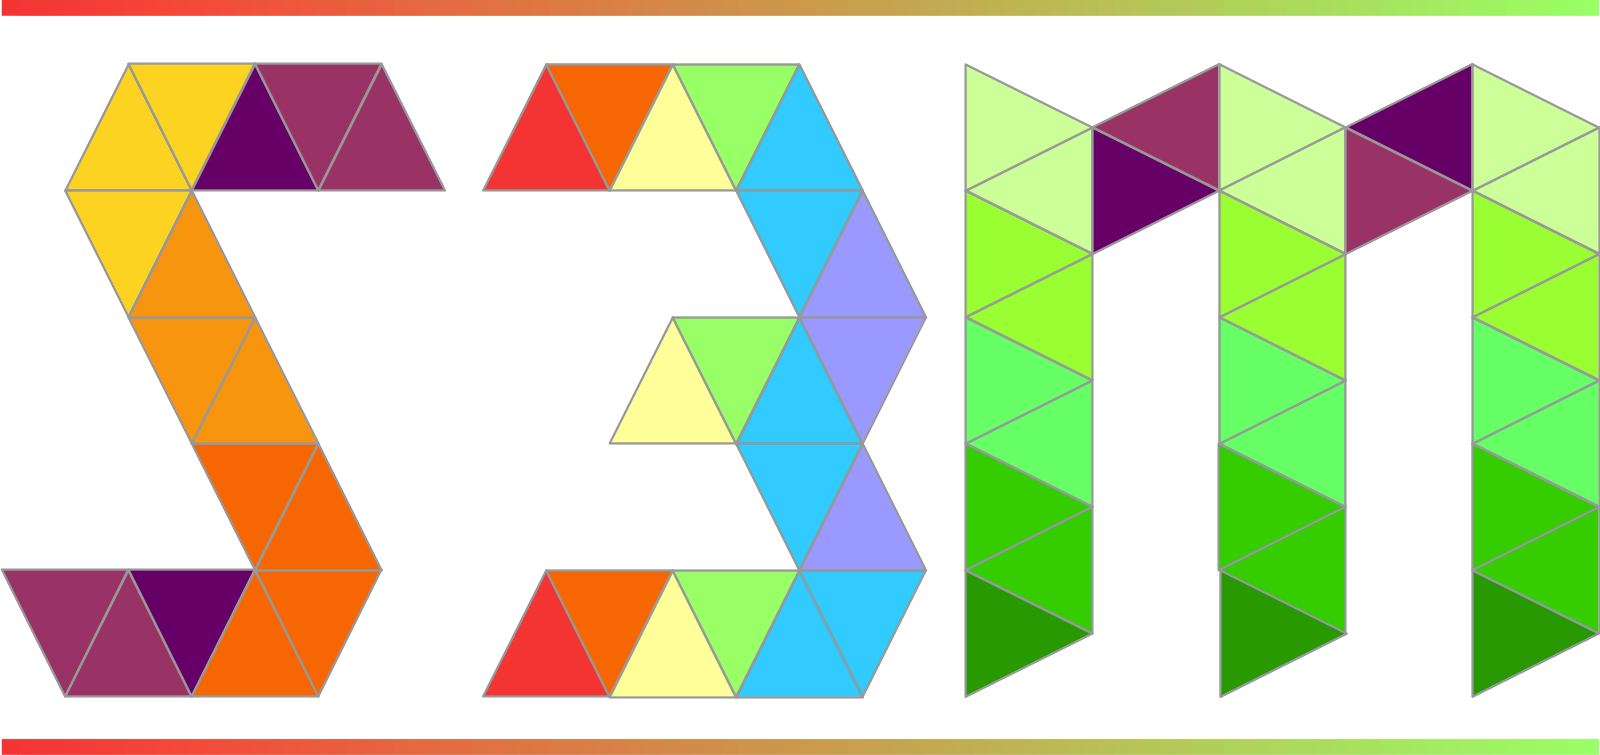
\includegraphics{figures/s3mlogo.png}

\hypertarget{introduction}{%
\chapter{Introduction}\label{introduction}}

The Simple Spatial Survey Method (S3M) was developed from the CSAS
coverage survey method as a response to the widespread adoption of
community management of acute malnutrition (CMAM) by ministries of
health. Large-scale programs need a large-scale survey method and S3M
was developed to meet that need.

S3M was designed to :

\begin{itemize}
\item
  Be simple enough for MoH, NGO, and UNO personnel without specialist
  statistical training to perform.
\item
  Provide a general survey method. S3M can be used to survey and map :

  \begin{itemize}
  \item
    Need for and coverage of selective-entry programs such as CMAM and
    TSFP as well as universal programs such as EPI, GMP, GFD (general
    ration), and ``blanket'' SFP over wide areas.
  \item
    Levels of indicators such as those for IYCF, WASH, and period
    prevalence / cumulative prevalence of ARI, fever, and diarrhoea over
    wide areas.
  \end{itemize}
\end{itemize}

This document concentrates on using S3M to assess the need for and
coverage of:

\begin{itemize}
\item
  Treatment of SAM in children aged between 6 and 59 months;
\item
  Vitamin A supplementation;
\item
  Micronutrient powder supplementation;
\item
  Ferrous sulfate-folic acid supplementation; and,
\item
  Infant and young child feeding counselling.
\end{itemize}

\hypertarget{sample}{%
\chapter{The survey sample}\label{sample}}

The survey method described here uses a two-stage sample:

\begin{itemize}
\item
  \textbf{First-stage:} We take an even (or near-even) spatial sample of
  communities from all of the communities in the survey area.
\item
  \textbf{Second-stage:} We take a sample of eligible individuals from
  each of the communities identified in the first stage of sampling.
\end{itemize}

Two-stage sampling is used in many survey methods. A typical example of
a survey method that uses a two-stage sample is the SMART method that is
commonly used for nutritional anthropometry surveys.

The main difference between the sample taken in S3M based surveys and in
SMART type surveys is that S3M based samples use a spatial sample in the
first stage whereas SMART type surveys use a proportional to population
size (PPS) sample.

The advantages of using a spatial first stage sample is that such a
sample allows us to identify where (and why) coverage is good, and where
(and why) coverage is poor. This information is essential to improving
program coverage and ensuring equitable access to services.

A spatial sample can be used to produce equivalent results to a
traditional proportional to population size (PPS) sample as is used in
(e.g.) SMART type surveys using a weighted analysis. This means that a
spatial sample can be made to act as a PPS sample. A PPS type sample
cannot, however, be made to act as a spatial sample.

\hypertarget{sample-size-considerations}{%
\section{Sample size considerations}\label{sample-size-considerations}}

In general, the sample size needed for proportion-type indicators such
as coverage can be calculated using the following equation.

\[\begin{aligned}
n & ~ = ~ Z^2 ~ \times ~ \frac{p(1 ~ - ~ p)}{c ^ 2} \\
\\
where: & \\
\\
Z & ~ = ~ \text{z-value for preferred confidence interval} \\
p & ~ = ~ \text{expected indicator proportion/prevalence} \\
c & ~ = ~ \text{level of precision}
\end{aligned}\]

The \(Z\) value is usually 1.96 for a 95\% confidence interval. The
\(p\) should usually be based on previous coverage results if available.
If not, it is usually appropriate to set \(p\) at 50\% (0.5) as this
results in the highest sample size estimate. The precision (\(c\)) for
coverage surveys is usually set at ±10\% based on standard precision
used for immunisation coverage.

Using these values, the typical sample size needed for coverage surveys
is about 96.

\[ n ~ = ~ 1.96^2 ~ \times ~ \frac{0.5(1 ~ - ~ 0.5)}{0.10 ^ 2} ~ \approx ~  96 \]

However, the survey design needs to be taken into account. A cluster
survey such as the one that is proposed for the Liberia S3M will need to
inflate sample sizes to account for the loss of variance due to the
cluster design. This inflation factor is called the \emph{design effect}
(\emph{DEFF}) which is based on the \emph{intracluster correlation
coefficient} (\emph{ICC}).

Generally, a \emph{DEFF} of 2 is used to multiply the sample size with
to account for the loss of variance. This would mean that a sample size
of 192 would be the target sample size.

The sample size required will also depend on the indicators being
assessed.

SAM treatment coverage can be demonstrated in the following equation:

\[ \text{SAM treatment coverage} ~ = ~ \frac{\text{SAM cases in treatment}}{\text{Total SAM cases}} \]

This indicator requires a sample of under 5 children who have SAM. SAM
children are rare (at most 3\% of the general population of children
under 5). This means that the universe population of SAM children is
small hence a finite population correction can be applied to sample size
calculations. At the same time, given the active adaptive case finding
approach that will be applied to finding SAM cases is know to be
exhaustive, \emph{DEFF} would generally be close to 1. Therefore, a
sample size of about 96 is generally big enough to estimate SAM
treatment coverage with a ±10\% precision.

For vitamin A supplementation, micronutrient powder supplementation,
IYCF counselling and ferrous sulfate-folic acid
supplementation\footnote{If pregnant women is chosen as the universe
  population for the ferrous sulfate-folic acide supplementation, the
  sample size requirements can be reduced given that the number of
  pregnant women will be finite population as well and an active and
  adaptive case finding method will need to be applied to find pregnant
  women.}, the sample size of 192 would be the target sample size.

\hypertarget{urban-and-rural-sample-considerations}{%
\section{Urban and rural sample
considerations}\label{urban-and-rural-sample-considerations}}

Currently, the requirements for the survey is to provide coverage
estimates for Montserrado rural districts and the whole Grand Bassa
county. Urban areas have been specifically excluded.

Given that urban areas would most likely have different characteristics
than rural areas, it is more reasonable to treat urban areas as a
separate survey area. If urban areas are to be sampled, then urben areas
should have its own sample with the same minimum sample size as
described above. The implication of this would be an extra survey for
each and every urban area to be assessed.

\hypertarget{stage1}{%
\chapter{The first stage sample}\label{stage1}}

\hypertarget{step-1-find-a-map}{%
\section{Step 1: Find a map}\label{step-1-find-a-map}}

The first step in a S3M survey is to find a map of the survey area. A
map showing the locations of all towns and villages in the survey area
is essential. Try to find a map showing the locations of all towns and
villages in the survey area. You may need to update the map to take into
account migration and displacement.

For the coverage survey of 2 counties in Liberia, it will be practical
and useful to have:

\begin{itemize}
\tightlist
\item
  A small scale-map (a wide area map but with poor detail) of the entire
  survey area for each of the 2 counties. If the counties are contiguous
  (i.e., share borders with each other), the small scale map can be of
  the two counties together. This map does not need to show the location
  of all towns and villages in the survey area but it gives a general
  idea of where the 2 counties are located and main towns and locations
  and roads. Figure \ref{fig:smallScaleMap} is a small scale map of
  Liberia showing counties, roads and main towns and locations. Figure
  \ref{fig:smallScaleMapCounty} is a small scale map of two counties
  showing all the districts within the county, roads and main towns and
  locations.
\end{itemize}

\newpage

\begin{figure}[H]

{\centering 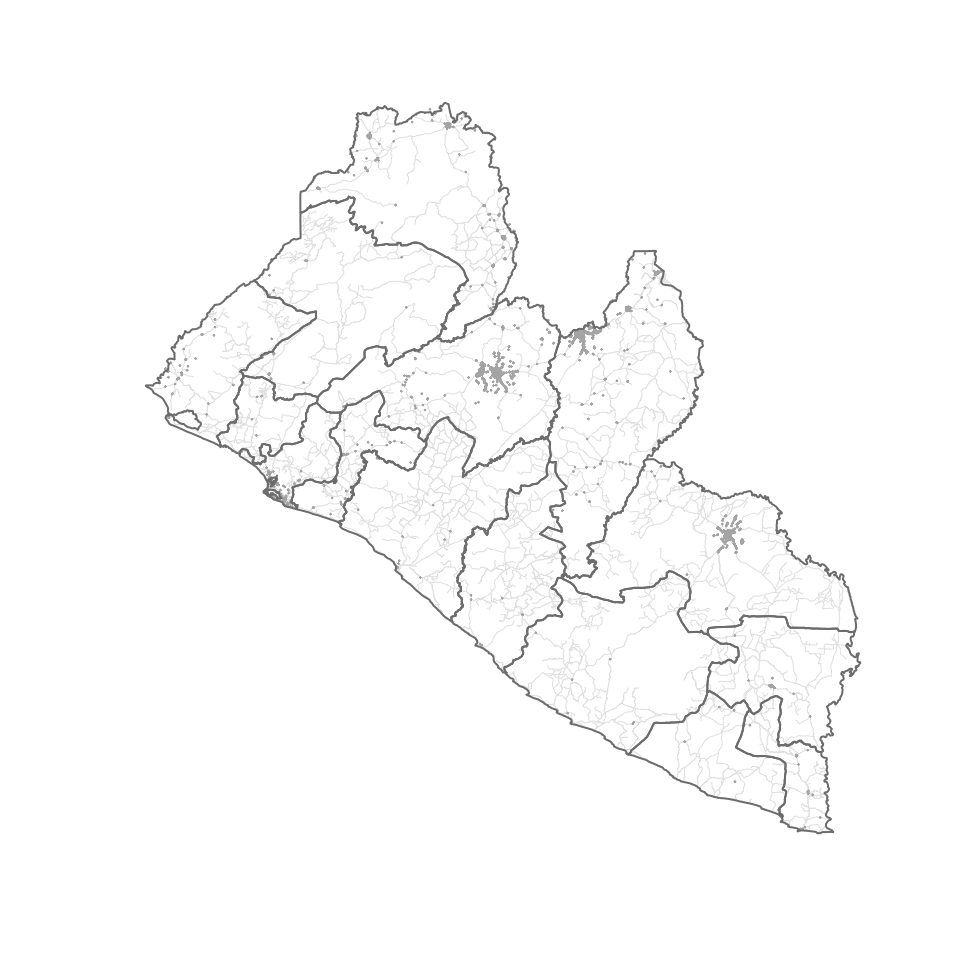
\includegraphics{figures/smallScaleMap-1} 

}

\caption{Small scale map of Liberia showing counties, roads and points of interest}\label{fig:smallScaleMap}
\end{figure}

\newpage

\begin{figure}[H]

{\centering 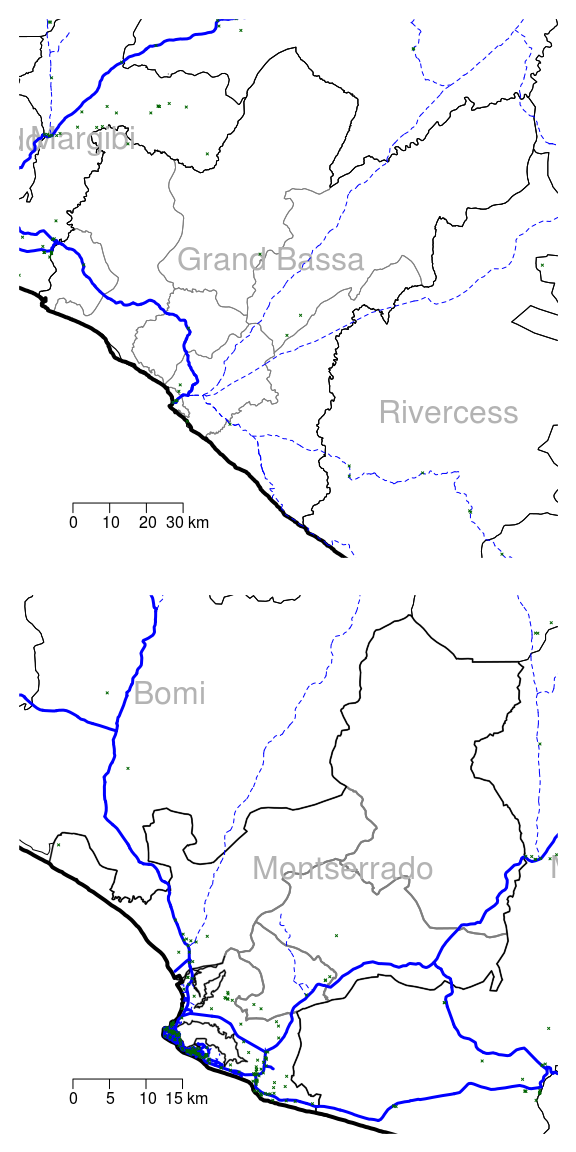
\includegraphics{figures/smallScaleMapCounty-1} 

}

\caption{Small scale map of Montserrado and Grand Bassa in Liberia showing all districts, roads and points of interest}\label{fig:smallScaleMapCounty}
\end{figure}

\newpage

\begin{itemize}
\tightlist
\item
  A collection of larger scale maps (a small area map but with good
  detail) of each of the selected counties and each of the districts
  within those counties in Liberia. Figure
  \ref{fig:largeScaleMapCounty1} is a large scale map of Montserrado
  county showing all districts, roads and all settlements. Figure
  \ref{fig:largeScaleMapDistricts1} is a collection of large scale maps
  of each of the districts of Montserrado country showing all roads and
  all settlements.
\end{itemize}

~

\begin{figure}[H]

{\centering 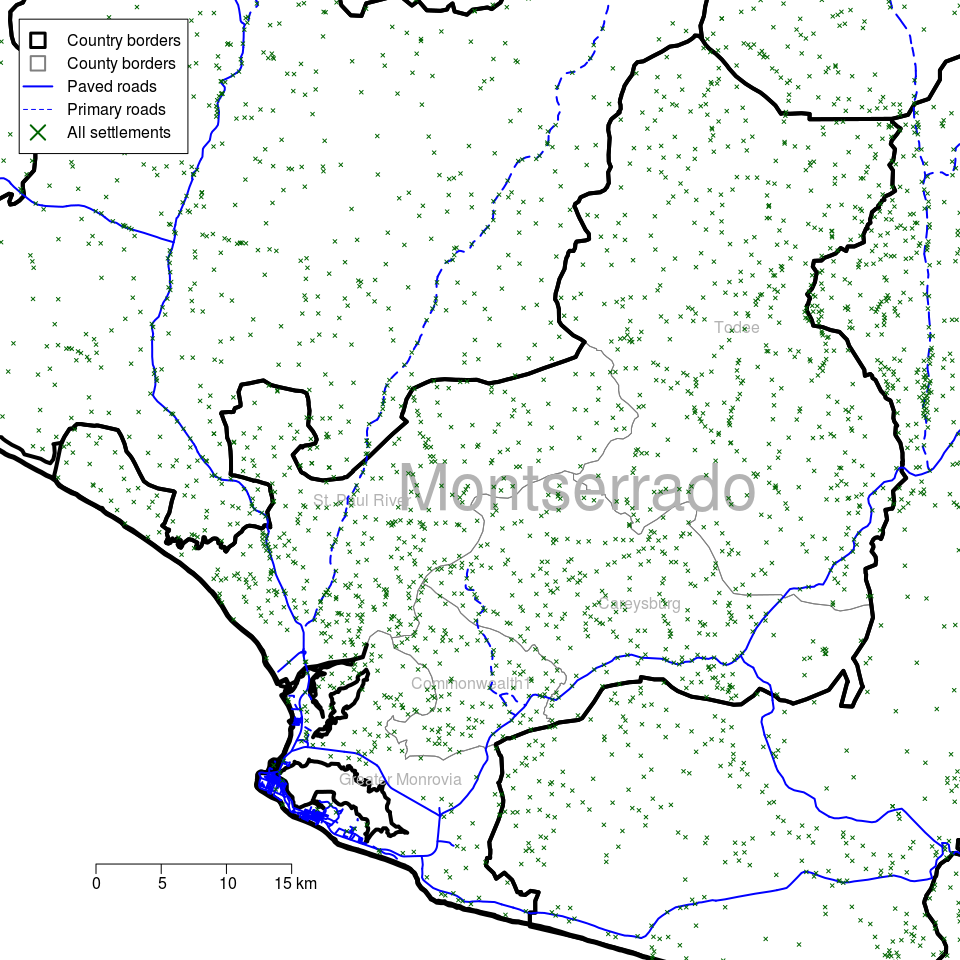
\includegraphics{figures/largeScaleMapCounty1-1} 

}

\caption{Large scale map of Montserrado county in Liberia showing all districts, roads and all settlements (towns, villages)}\label{fig:largeScaleMapCounty1}
\end{figure}

\newpage

\begin{figure}[H]

{\centering 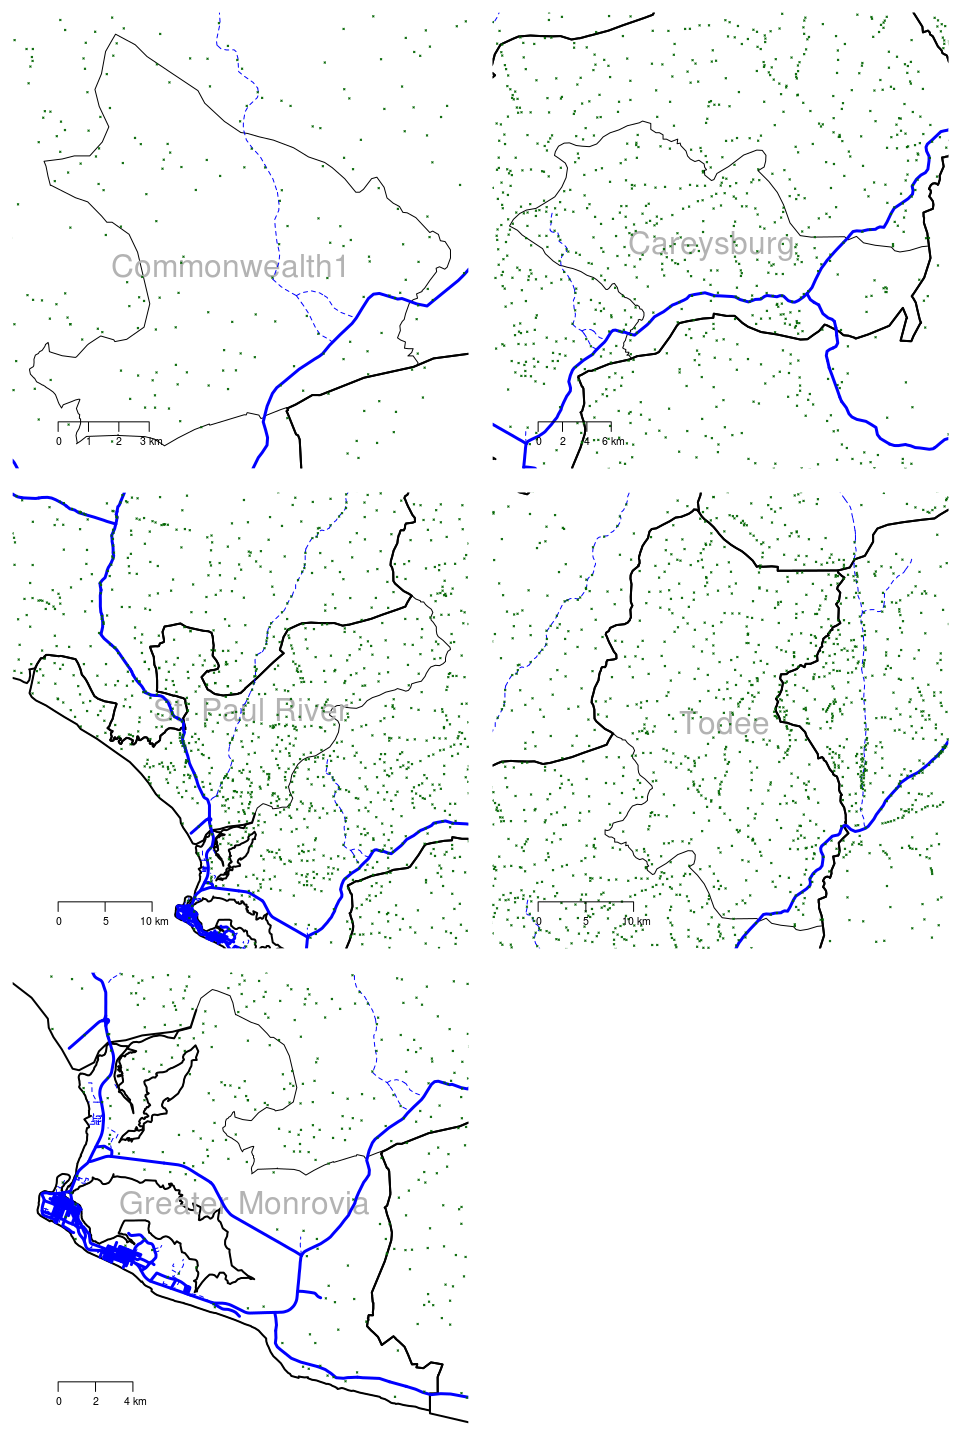
\includegraphics{figures/largeScaleMapDistricts1-1} 

}

\caption{Large scale maps of 5 districts of Montserrado county in Liberia showing roads and all settlements (towns, villages)}\label{fig:largeScaleMapDistricts1}
\end{figure}

\newpage

\begin{figure}[H]

{\centering 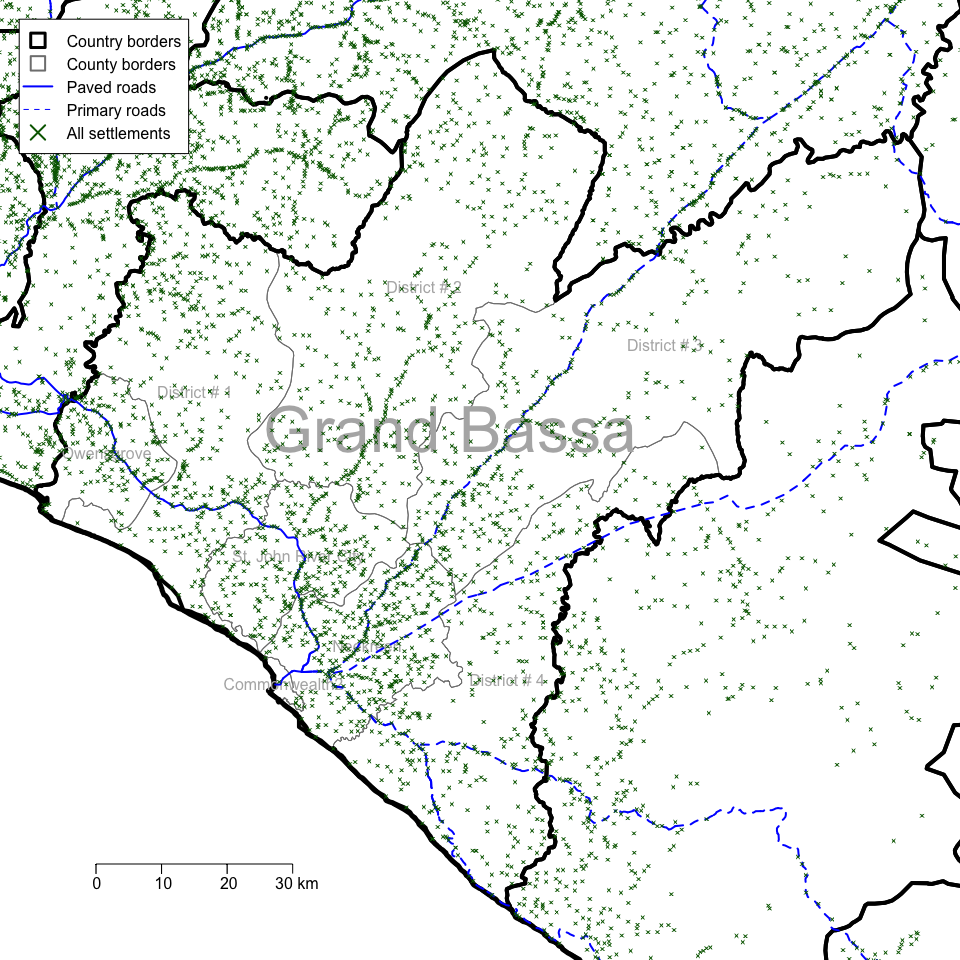
\includegraphics{figures/largeScaleMapCounty2-1} 

}

\caption{Large scale map of Grand Bassa county in Liberia showing all districts, roads and all settlements (towns, villages)}\label{fig:largeScaleMapCounty2}
\end{figure}

\newpage

\begin{figure}[H]

{\centering 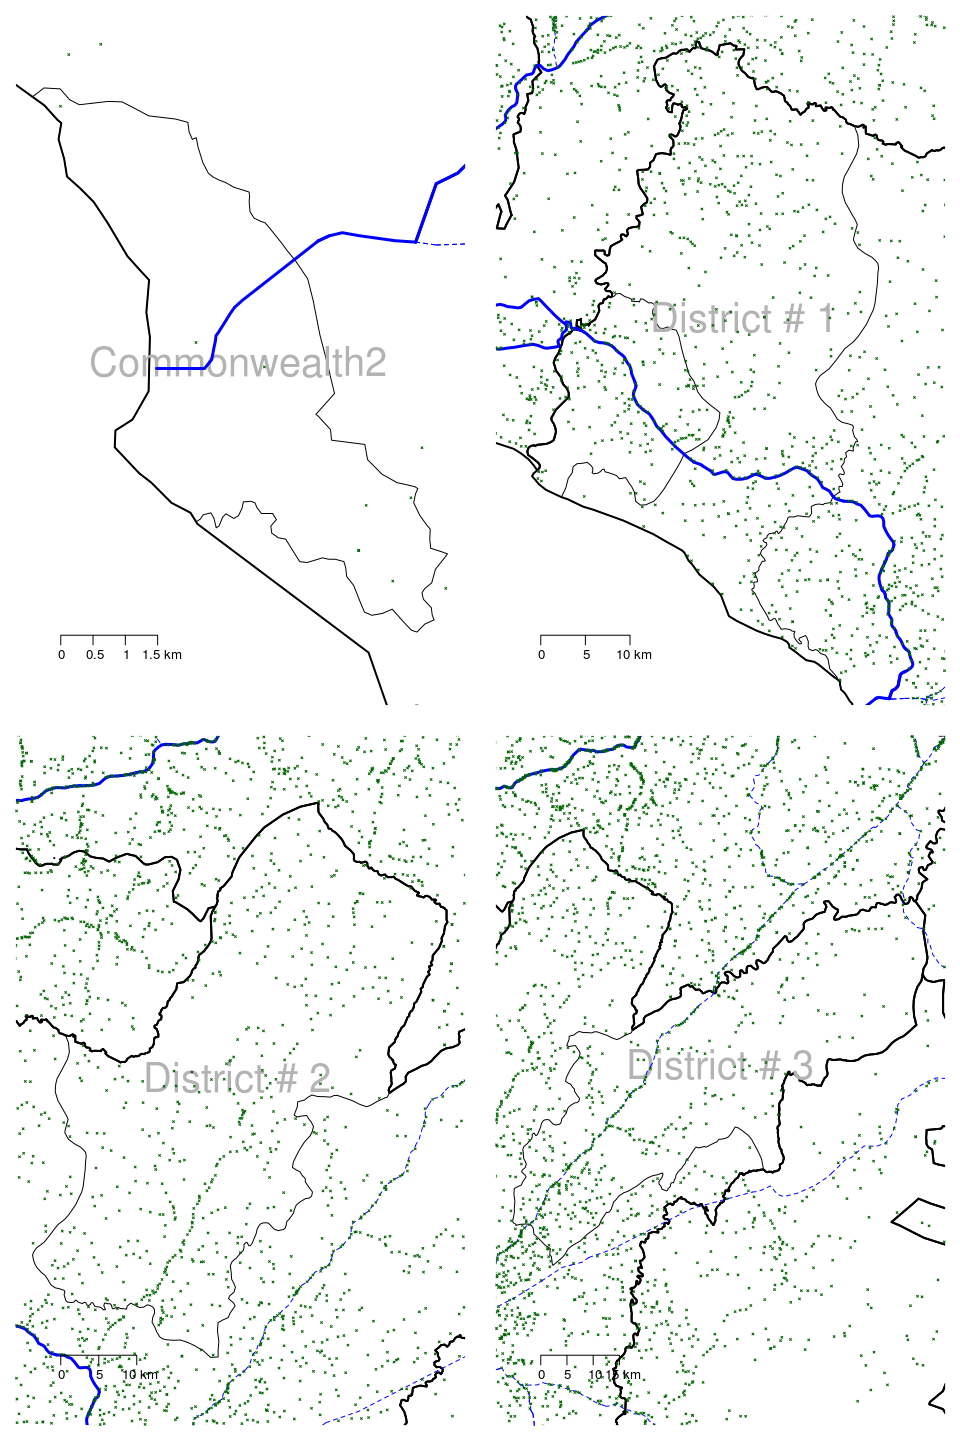
\includegraphics{figures/largeScaleMapDistricts2-1} 

}

\caption{Large scale maps of 8 districts of Grand Bassa county in Liberia showing roads and all settlements (towns, villages)}\label{fig:largeScaleMapDistricts2}
\end{figure}

\newpage

\begin{figure}[H]

{\centering 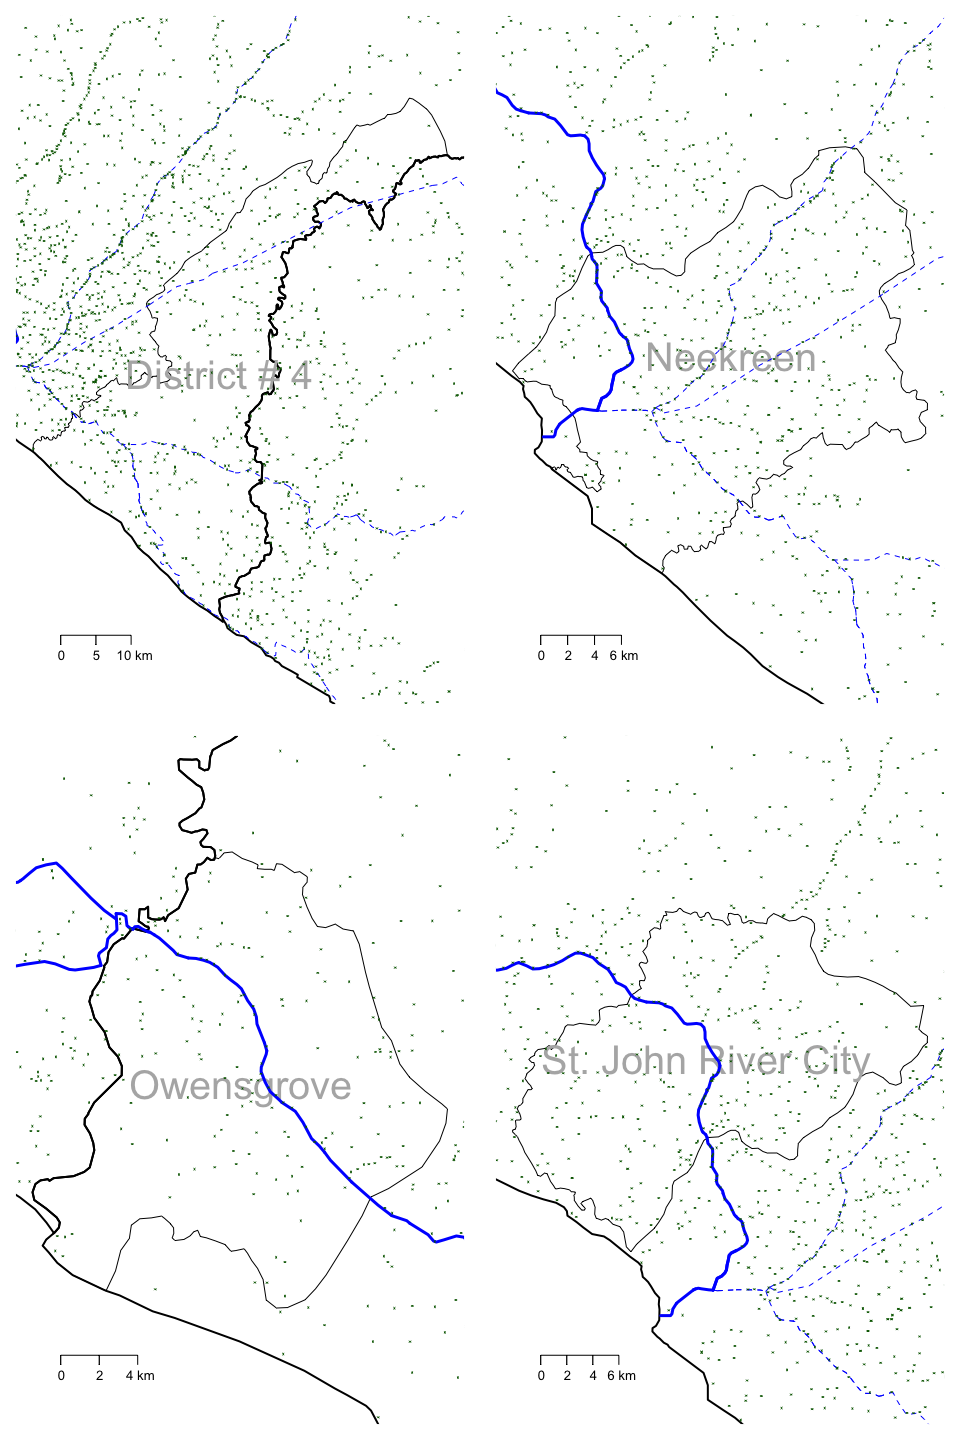
\includegraphics{figures/largeScaleMapDistricts3-1} 

}

\caption{Large scale maps of 8 districts of Grand Bassa county in Liberia showing roads and all settlements (towns, villages) continued}\label{fig:largeScaleMapDistricts3}
\end{figure}

\newpage

The small-scale maps in Figures \ref{fig:smallScaleMap} and
\ref{fig:smallScaleMapCounty} will be useful for identifying initial
sampling locations.

The large-scale maps in Figures \ref{fig:largeScaleMapCounty1},
\ref{fig:largeScaleMapCounty2}, \ref{fig:largeScaleMapDistricts1},
\ref{fig:largeScaleMapDistricts2} and \ref{fig:largeScaleMapDistricts3}
will be useful for identifying the precise location of sampling points
and for selecting the communities to be sampled.

\newpage

\hypertarget{step-2-decide-the-area-to-represent-each-sampling-point}{%
\section{Step 2: Decide the area to represent each sampling
point}\label{step-2-decide-the-area-to-represent-each-sampling-point}}

The easiest way of thinking about this is as a function of the intended
maximum distance (\(d\)) of any community from the nearest sampling
point (see Figure \ref{fig:distance1}.

~

\begin{figure}[H]

{\centering 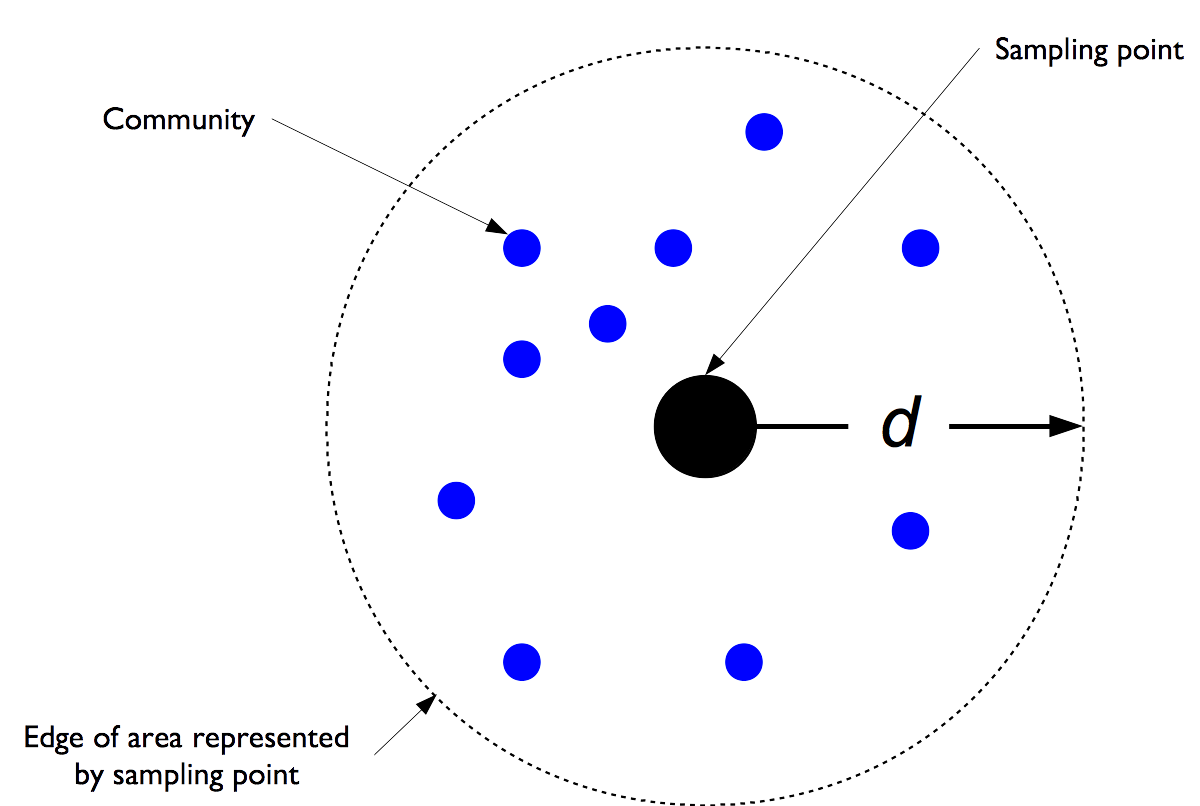
\includegraphics[width=16.67in]{figures/step2} 

}

\caption{Conceptual presentation of the area represented by each sampling point}\label{fig:distance1}
\end{figure}

~

There are other ways of thinking about \(d\). These are:

\begin{enumerate}
\def\labelenumi{\arabic{enumi}.}
\tightlist
\item
  \textbf{The area of each triangular tile}: This can be calculated
  using the formula:
\end{enumerate}

\[ A ~ = ~ \tan30^ \circ ~ \times ~ \frac{9}{4} ~ d ^ 2 \]

For \(d ~ = ~ 10 ~ \text{km}\) the area of each triangular tile will be
about:

\[ A ~ = ~ \tan30^ \circ ~ \times ~ \frac{9}{4} ~ d ^ 2 ~ \approx ~ 1.3 ~ \times ~ 100 ~ = ~ 130 ~ \text{km} ^ 2 \]

\begin{enumerate}
\def\labelenumi{\arabic{enumi}.}
\setcounter{enumi}{1}
\tightlist
\item
  \textbf{Practicability}: Most of the time spent in the field when
  doing a survey will be in travelling to and from sampling points.
  Having many sampling points can make for an expensive and / or lengthy
  survey. If you know how many sampling points that you can afford to
  take (\(m\)) then you can make a \textbf{very approximate} estimate of
  a suitable value for d using the following \emph{rule-of-thumb}
  formula:
\end{enumerate}

\[ d ~ \approx ~ \sqrt{\frac{\text{Program Area}}{m}} \]

The value of \(d\) calculated using this formula is approximate and
should be used as a starting point for a number of trial samples using
the procedure outlined below.

~

\begin{longtable}[]{@{}cccc@{}}
\toprule
\begin{minipage}[b]{0.14\columnwidth}\centering
\textbf{Pair}\strut
\end{minipage} & \begin{minipage}[b]{0.20\columnwidth}\centering
\textbf{Distance}\strut
\end{minipage} & \begin{minipage}[b]{0.14\columnwidth}\centering
\textbf{Pair}\strut
\end{minipage} & \begin{minipage}[b]{0.20\columnwidth}\centering
\textbf{Distance}\strut
\end{minipage}\tabularnewline
\midrule
\endhead
\begin{minipage}[t]{0.14\columnwidth}\centering
1\strut
\end{minipage} & \begin{minipage}[t]{0.20\columnwidth}\centering
21 km\strut
\end{minipage} & \begin{minipage}[t]{0.14\columnwidth}\centering
13\strut
\end{minipage} & \begin{minipage}[t]{0.20\columnwidth}\centering
13 km\strut
\end{minipage}\tabularnewline
\begin{minipage}[t]{0.14\columnwidth}\centering
2\strut
\end{minipage} & \begin{minipage}[t]{0.20\columnwidth}\centering
14 km\strut
\end{minipage} & \begin{minipage}[t]{0.14\columnwidth}\centering
14\strut
\end{minipage} & \begin{minipage}[t]{0.20\columnwidth}\centering
11 km\strut
\end{minipage}\tabularnewline
\begin{minipage}[t]{0.14\columnwidth}\centering
3\strut
\end{minipage} & \begin{minipage}[t]{0.20\columnwidth}\centering
13 km\strut
\end{minipage} & \begin{minipage}[t]{0.14\columnwidth}\centering
15\strut
\end{minipage} & \begin{minipage}[t]{0.20\columnwidth}\centering
12 km\strut
\end{minipage}\tabularnewline
\begin{minipage}[t]{0.14\columnwidth}\centering
4\strut
\end{minipage} & \begin{minipage}[t]{0.20\columnwidth}\centering
17 km\strut
\end{minipage} & \begin{minipage}[t]{0.14\columnwidth}\centering
16\strut
\end{minipage} & \begin{minipage}[t]{0.20\columnwidth}\centering
15 km\strut
\end{minipage}\tabularnewline
\begin{minipage}[t]{0.14\columnwidth}\centering
5\strut
\end{minipage} & \begin{minipage}[t]{0.20\columnwidth}\centering
11 km\strut
\end{minipage} & \begin{minipage}[t]{0.14\columnwidth}\centering
17\strut
\end{minipage} & \begin{minipage}[t]{0.20\columnwidth}\centering
13 km\strut
\end{minipage}\tabularnewline
\begin{minipage}[t]{0.14\columnwidth}\centering
6\strut
\end{minipage} & \begin{minipage}[t]{0.20\columnwidth}\centering
14 km\strut
\end{minipage} & \begin{minipage}[t]{0.14\columnwidth}\centering
18\strut
\end{minipage} & \begin{minipage}[t]{0.20\columnwidth}\centering
16 km\strut
\end{minipage}\tabularnewline
\begin{minipage}[t]{0.14\columnwidth}\centering
7\strut
\end{minipage} & \begin{minipage}[t]{0.20\columnwidth}\centering
12 km\strut
\end{minipage} & \begin{minipage}[t]{0.14\columnwidth}\centering
19\strut
\end{minipage} & \begin{minipage}[t]{0.20\columnwidth}\centering
18 km\strut
\end{minipage}\tabularnewline
\begin{minipage}[t]{0.14\columnwidth}\centering
8\strut
\end{minipage} & \begin{minipage}[t]{0.20\columnwidth}\centering
15 km\strut
\end{minipage} & \begin{minipage}[t]{0.14\columnwidth}\centering
20\strut
\end{minipage} & \begin{minipage}[t]{0.20\columnwidth}\centering
13 km\strut
\end{minipage}\tabularnewline
\begin{minipage}[t]{0.14\columnwidth}\centering
9\strut
\end{minipage} & \begin{minipage}[t]{0.20\columnwidth}\centering
16 km\strut
\end{minipage} & \begin{minipage}[t]{0.14\columnwidth}\centering
21\strut
\end{minipage} & \begin{minipage}[t]{0.20\columnwidth}\centering
8 km\strut
\end{minipage}\tabularnewline
\begin{minipage}[t]{0.14\columnwidth}\centering
10\strut
\end{minipage} & \begin{minipage}[t]{0.20\columnwidth}\centering
12 km\strut
\end{minipage} & \begin{minipage}[t]{0.14\columnwidth}\centering
22\strut
\end{minipage} & \begin{minipage}[t]{0.20\columnwidth}\centering
16 km\strut
\end{minipage}\tabularnewline
\begin{minipage}[t]{0.14\columnwidth}\centering
11\strut
\end{minipage} & \begin{minipage}[t]{0.20\columnwidth}\centering
17 km\strut
\end{minipage} & \begin{minipage}[t]{0.14\columnwidth}\centering
23\strut
\end{minipage} & \begin{minipage}[t]{0.20\columnwidth}\centering
18 km\strut
\end{minipage}\tabularnewline
\begin{minipage}[t]{0.14\columnwidth}\centering
12\strut
\end{minipage} & \begin{minipage}[t]{0.20\columnwidth}\centering
14 km\strut
\end{minipage} & \begin{minipage}[t]{0.14\columnwidth}\centering
24\strut
\end{minipage} & \begin{minipage}[t]{0.20\columnwidth}\centering
14 km\strut
\end{minipage}\tabularnewline
\bottomrule
\end{longtable}

~

\begin{figure}[H]

{\centering 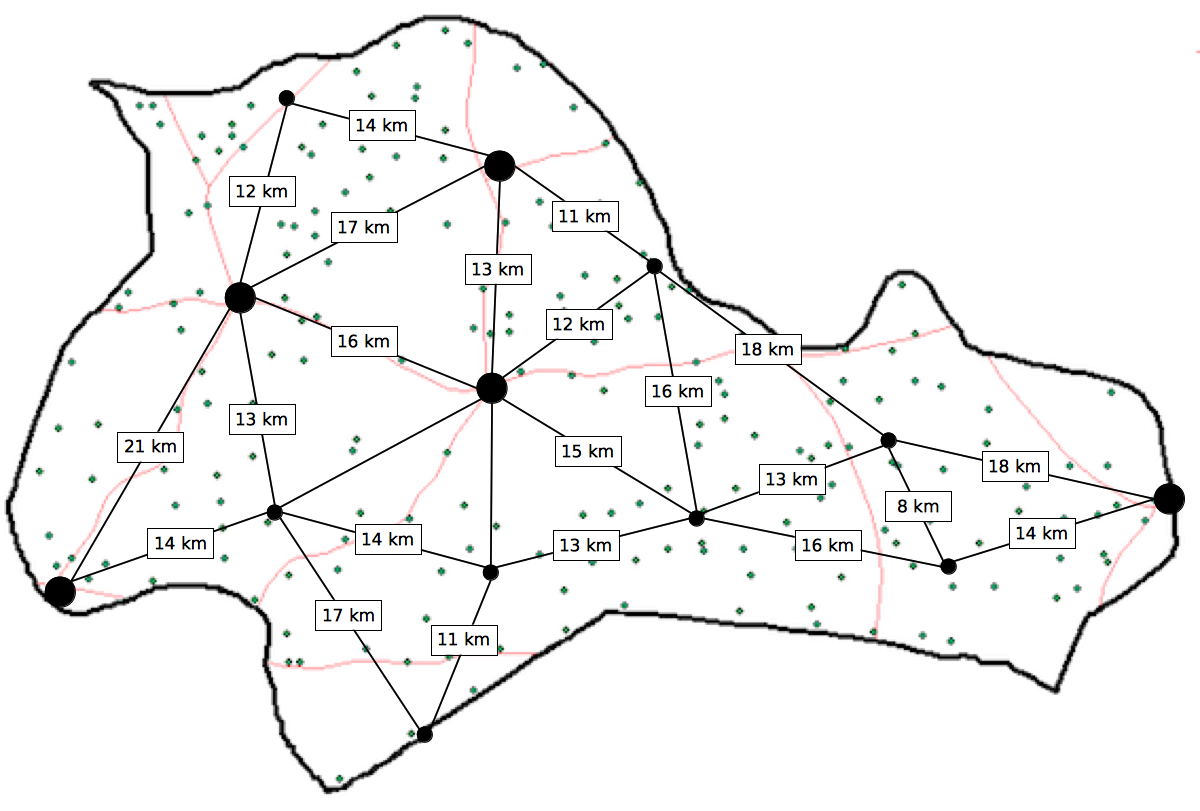
\includegraphics[width=16.67in]{figures/step2a} 

}

\caption{Distances of communities to the nearest substantial markets}\label{fig:distance2}
\end{figure}

~

\BeginKnitrBlock{rmdcalc}
Following are steps to estimate value of \(d\) based on distances that
carers are willing or able to walk to access services.

~

Using the information from the distance table, add the distances
together:

\[ \sum \text{Distance} ~ = ~ 343 ~ \text{km} \]

~

Divide the result by the number of paired distances:

\[ \frac{\sum \text{Distance}}{\text{Number of paired distances}} ~ = ~ \frac{343}{24} ~ = ~ 14.29 ~ \text{km} \]

~

Divide the result by two:

\[ d ~ = ~ \frac{14.29}{2} ~ = ~ 7.15 ~ \approx ~ 7 ~ \text{km} \]
\EndKnitrBlock{rmdcalc}

~

This is an estimate of the distance that carers are willing or able to
walk to access services. Only distances between towns and villages with
markets are used in this calculation.

A way of deciding a value for \(d\) that is based on the economic
geography of the survey area is to set \(d\) to one half of the mean
distance between neighbouring pairs of communities with substantial
markets.

S3M surveys have been done using a wide range (i.e.~from
\(d ~ = ~ 8 ~ \text{km}\) to \(d ~ = ~ 33 ~ \text{km}\)) of values for
\(d\). A value for \(d\) of 10 km or 12 km will probably be small enough
in most circumstances.

\newpage

\hypertarget{step-3-draw-a-grid-over-the-map}{%
\section{Step 3: Draw a grid over the
map}\label{step-3-draw-a-grid-over-the-map}}

\begin{figure}[H]

{\centering 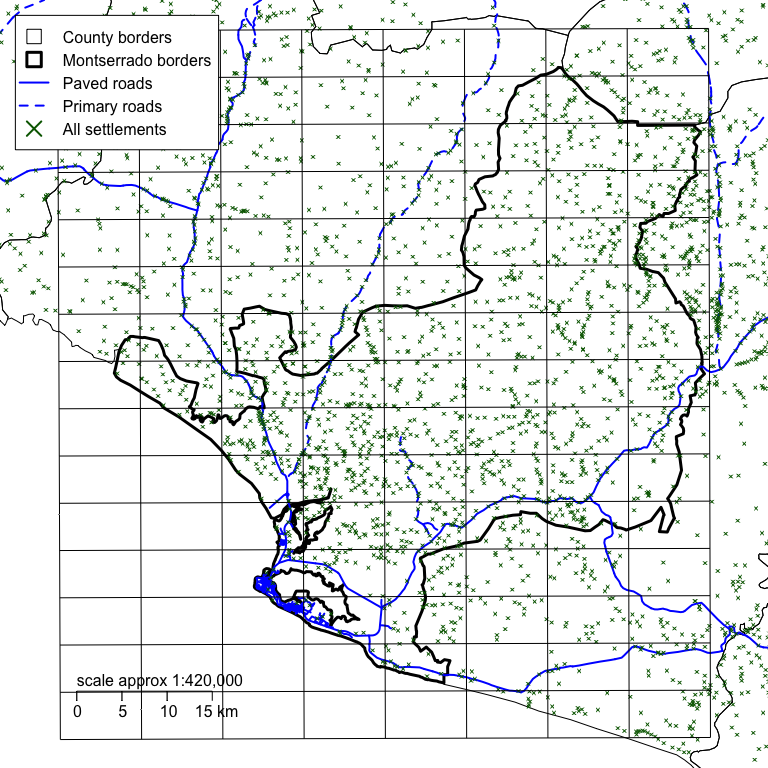
\includegraphics{figures/grid1-1} 

}

\caption{Montserrado county with a rectangular grid defined by d of 6 km}\label{fig:grid1}
\end{figure}

\newpage

\begin{figure}[H]

{\centering 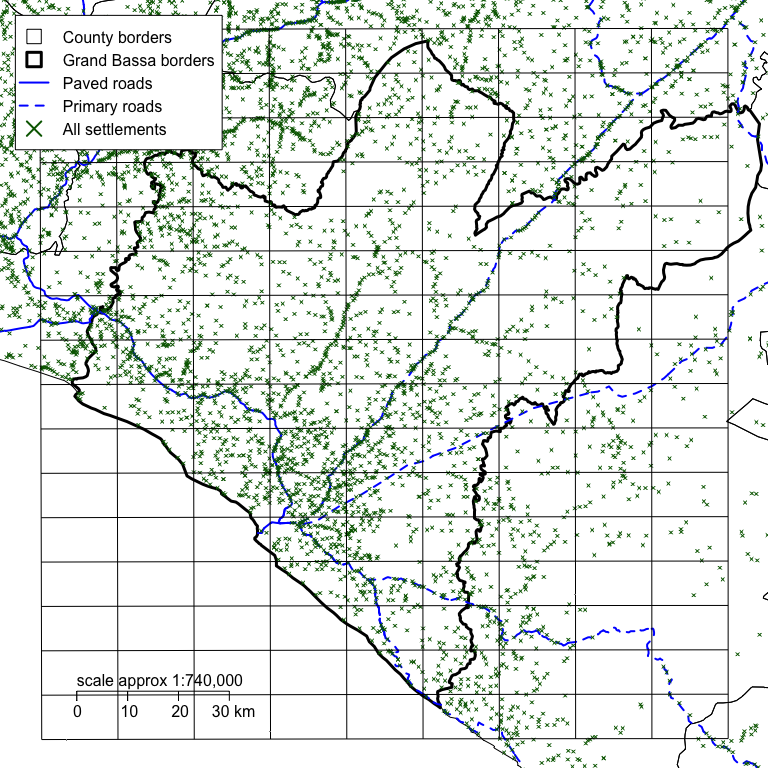
\includegraphics{figures/grid1a-1} 

}

\caption{Grand Bassa county with a rectangular grid defined by d of 10 km}\label{fig:grid1a}
\end{figure}

~

The next step is to draw a grid over the map.

The size of the grid is determined by the distance (\(d\)) that you
decided in \textbf{Step 2}.

The grid is rectangular rather than square. This allows us to place
sampling points at the centres of hexagons in a hexagonal grid without
the need to draw a hexagonal grid (see \textbf{Step 4}).

The width of the grid in the east-west (\(x\)) direction is different
from the height of the grid in the north-south (\(y\)) direction.

The width of the grid in the east-west (\(x\)) direction is calculated
using:

\[ x ~ = ~ \frac{3d}{2} \]

where \(d\) is the distance (\(d\)) that you decided in \textbf{Step 2}.

The height of the grid in the north-south (\(y\)) direction can be
calculated using:

\[ y ~ = ~ \frac{\sqrt{3}d}{2} \]

where \(d\) is the distance (\(d\)) that you decided in \textbf{Step 2}.

For example, in Figure \ref{fig:grid1}, we used
\(d ~ = ~ 6 ~ \text{km}\). This value of \(d\) creates a rectangular
grid with the following dimensions:

\[ x ~ = ~ \frac{3d}{2} ~ = ~ \frac{3 ~ \times ~ 6}{2} ~ = ~ \frac{18}{2} ~ = ~ 9 ~ \text{km} \]

and:

\[ y ~ = ~ \frac{\sqrt{3}d}{2} ~ \approx ~ \frac{1.73 ~ \times ~ 6}{2} ~ \approx ~ \frac{10.38}{2} ~ \approx ~ 5.2 ~ \text{km} \]

So, the grid in Figure \ref{fig:grid1} is 9 km long on the east-west
direction and 5.2 km on the north and south direction.

\newpage

The table below shows the grid sizes for different values of \(d\):

\begin{longtable}[]{@{}rrrlrrr@{}}
\toprule
\begin{minipage}[b]{0.10\columnwidth}\raggedleft
\textbf{d}\strut
\end{minipage} & \begin{minipage}[b]{0.14\columnwidth}\raggedleft
\textbf{x}\strut
\end{minipage} & \begin{minipage}[b]{0.14\columnwidth}\raggedleft
\textbf{y}\strut
\end{minipage} & \begin{minipage}[b]{0.06\columnwidth}\raggedright
\strut
\end{minipage} & \begin{minipage}[b]{0.10\columnwidth}\raggedleft
\textbf{d}\strut
\end{minipage} & \begin{minipage}[b]{0.14\columnwidth}\raggedleft
\textbf{x}\strut
\end{minipage} & \begin{minipage}[b]{0.14\columnwidth}\raggedleft
\textbf{y}\strut
\end{minipage}\tabularnewline
\midrule
\endhead
\begin{minipage}[t]{0.10\columnwidth}\raggedleft
5\strut
\end{minipage} & \begin{minipage}[t]{0.14\columnwidth}\raggedleft
7.5\strut
\end{minipage} & \begin{minipage}[t]{0.14\columnwidth}\raggedleft
4.3\strut
\end{minipage} & \begin{minipage}[t]{0.06\columnwidth}\raggedright
\strut
\end{minipage} & \begin{minipage}[t]{0.10\columnwidth}\raggedleft
13\strut
\end{minipage} & \begin{minipage}[t]{0.14\columnwidth}\raggedleft
19.5\strut
\end{minipage} & \begin{minipage}[t]{0.14\columnwidth}\raggedleft
11.3\strut
\end{minipage}\tabularnewline
\begin{minipage}[t]{0.10\columnwidth}\raggedleft
6\strut
\end{minipage} & \begin{minipage}[t]{0.14\columnwidth}\raggedleft
9.0\strut
\end{minipage} & \begin{minipage}[t]{0.14\columnwidth}\raggedleft
5.2\strut
\end{minipage} & \begin{minipage}[t]{0.06\columnwidth}\raggedright
\strut
\end{minipage} & \begin{minipage}[t]{0.10\columnwidth}\raggedleft
14\strut
\end{minipage} & \begin{minipage}[t]{0.14\columnwidth}\raggedleft
21.0\strut
\end{minipage} & \begin{minipage}[t]{0.14\columnwidth}\raggedleft
12.1\strut
\end{minipage}\tabularnewline
\begin{minipage}[t]{0.10\columnwidth}\raggedleft
7\strut
\end{minipage} & \begin{minipage}[t]{0.14\columnwidth}\raggedleft
10.5\strut
\end{minipage} & \begin{minipage}[t]{0.14\columnwidth}\raggedleft
6.1\strut
\end{minipage} & \begin{minipage}[t]{0.06\columnwidth}\raggedright
\strut
\end{minipage} & \begin{minipage}[t]{0.10\columnwidth}\raggedleft
15\strut
\end{minipage} & \begin{minipage}[t]{0.14\columnwidth}\raggedleft
22.5\strut
\end{minipage} & \begin{minipage}[t]{0.14\columnwidth}\raggedleft
13.0\strut
\end{minipage}\tabularnewline
\begin{minipage}[t]{0.10\columnwidth}\raggedleft
8\strut
\end{minipage} & \begin{minipage}[t]{0.14\columnwidth}\raggedleft
12.0\strut
\end{minipage} & \begin{minipage}[t]{0.14\columnwidth}\raggedleft
6.9\strut
\end{minipage} & \begin{minipage}[t]{0.06\columnwidth}\raggedright
\strut
\end{minipage} & \begin{minipage}[t]{0.10\columnwidth}\raggedleft
16\strut
\end{minipage} & \begin{minipage}[t]{0.14\columnwidth}\raggedleft
24.0\strut
\end{minipage} & \begin{minipage}[t]{0.14\columnwidth}\raggedleft
13.9\strut
\end{minipage}\tabularnewline
\begin{minipage}[t]{0.10\columnwidth}\raggedleft
9\strut
\end{minipage} & \begin{minipage}[t]{0.14\columnwidth}\raggedleft
13,5\strut
\end{minipage} & \begin{minipage}[t]{0.14\columnwidth}\raggedleft
7.8\strut
\end{minipage} & \begin{minipage}[t]{0.06\columnwidth}\raggedright
\strut
\end{minipage} & \begin{minipage}[t]{0.10\columnwidth}\raggedleft
17\strut
\end{minipage} & \begin{minipage}[t]{0.14\columnwidth}\raggedleft
25.5\strut
\end{minipage} & \begin{minipage}[t]{0.14\columnwidth}\raggedleft
14.7\strut
\end{minipage}\tabularnewline
\begin{minipage}[t]{0.10\columnwidth}\raggedleft
10\strut
\end{minipage} & \begin{minipage}[t]{0.14\columnwidth}\raggedleft
15.0\strut
\end{minipage} & \begin{minipage}[t]{0.14\columnwidth}\raggedleft
8.7\strut
\end{minipage} & \begin{minipage}[t]{0.06\columnwidth}\raggedright
\strut
\end{minipage} & \begin{minipage}[t]{0.10\columnwidth}\raggedleft
18\strut
\end{minipage} & \begin{minipage}[t]{0.14\columnwidth}\raggedleft
27.0\strut
\end{minipage} & \begin{minipage}[t]{0.14\columnwidth}\raggedleft
15.6\strut
\end{minipage}\tabularnewline
\begin{minipage}[t]{0.10\columnwidth}\raggedleft
11\strut
\end{minipage} & \begin{minipage}[t]{0.14\columnwidth}\raggedleft
16.5\strut
\end{minipage} & \begin{minipage}[t]{0.14\columnwidth}\raggedleft
19.5\strut
\end{minipage} & \begin{minipage}[t]{0.06\columnwidth}\raggedright
\strut
\end{minipage} & \begin{minipage}[t]{0.10\columnwidth}\raggedleft
19\strut
\end{minipage} & \begin{minipage}[t]{0.14\columnwidth}\raggedleft
28.5\strut
\end{minipage} & \begin{minipage}[t]{0.14\columnwidth}\raggedleft
16.5\strut
\end{minipage}\tabularnewline
\begin{minipage}[t]{0.10\columnwidth}\raggedleft
12\strut
\end{minipage} & \begin{minipage}[t]{0.14\columnwidth}\raggedleft
18.0\strut
\end{minipage} & \begin{minipage}[t]{0.14\columnwidth}\raggedleft
10.4\strut
\end{minipage} & \begin{minipage}[t]{0.06\columnwidth}\raggedright
\strut
\end{minipage} & \begin{minipage}[t]{0.10\columnwidth}\raggedleft
20\strut
\end{minipage} & \begin{minipage}[t]{0.14\columnwidth}\raggedleft
30.0\strut
\end{minipage} & \begin{minipage}[t]{0.14\columnwidth}\raggedleft
17.3\strut
\end{minipage}\tabularnewline
\bottomrule
\end{longtable}

When drawing the grid make sure that it covers the entire survey area.

It is usually best to draw a grid that covers an area that is a little
larger than the entire survey area. This helps to ensure that the survey
will sample from the entire survey area.

The grid can be drawn using marker pens onto plastic film overlaying the
map. This protects the map and allows you to reposition the grid to
improve the coverage of the sample should this be needed.

If you are drawing the grid directly onto the map then use a soft pencil
(e.g.~a \emph{2B} or \emph{\#1} pencil). A soft pencil will not damage
the surface of the map and is easy to erase using a soft rubber eraser
should you make a mistake or need to draw a different grid.

\newpage

\hypertarget{step-4-create-an-even-spread-of-sampling-points}{%
\section{Step 4: Create an even spread of sampling
points}\label{step-4-create-an-even-spread-of-sampling-points}}

\begin{figure}[H]

{\centering 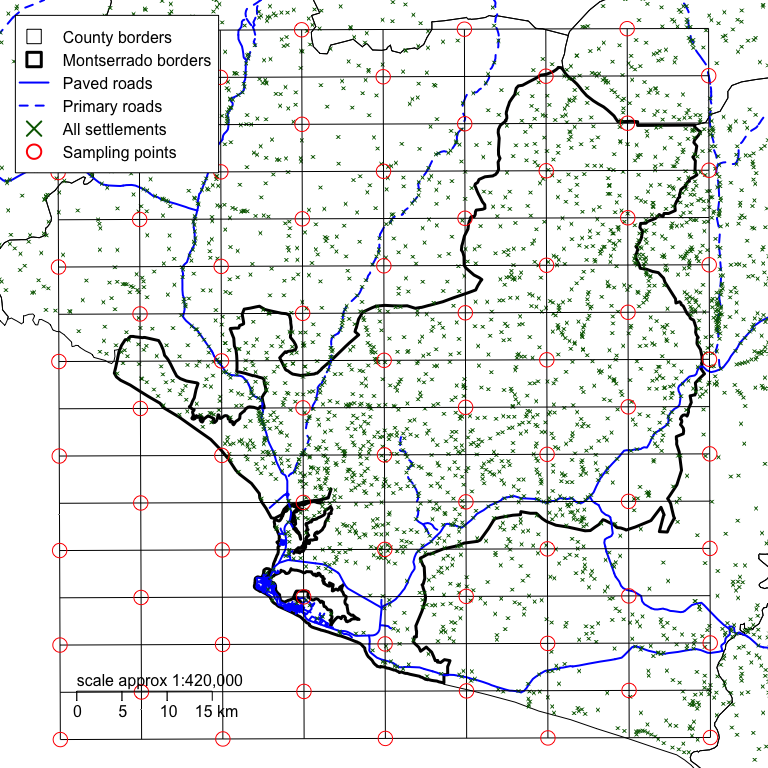
\includegraphics{figures/grid2-1} 

}

\caption{Montserrado county with a rectangular grid defined by d of 6 km and alternating intersections of the grid used to identify sampling points}\label{fig:grid2}
\end{figure}

\newpage

\begin{figure}[H]

{\centering 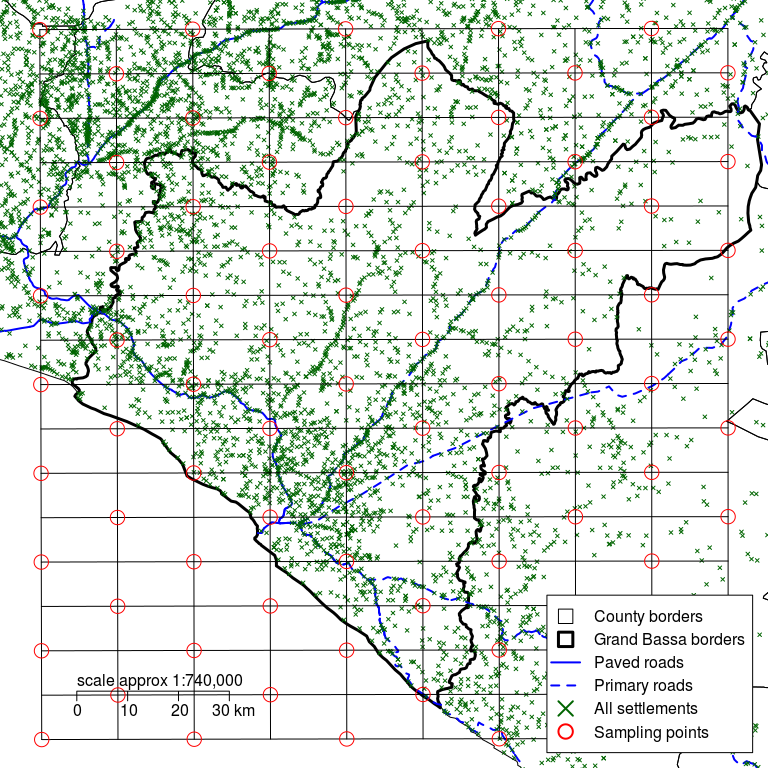
\includegraphics{figures/grid2a-1} 

}

\caption{Grand Bassa county with a rectangular grid defined by d of 10 km and alternating intersections of the grid used to identify sampling points}\label{fig:grid2a}
\end{figure}

Sampling points are located at the intersections of the rectangular grid
in a staggered fashion. Alternate intersections of the grid in the x
(east-west) and y (north-south) directions are used:

\newpage

\begin{figure}[H]

{\centering 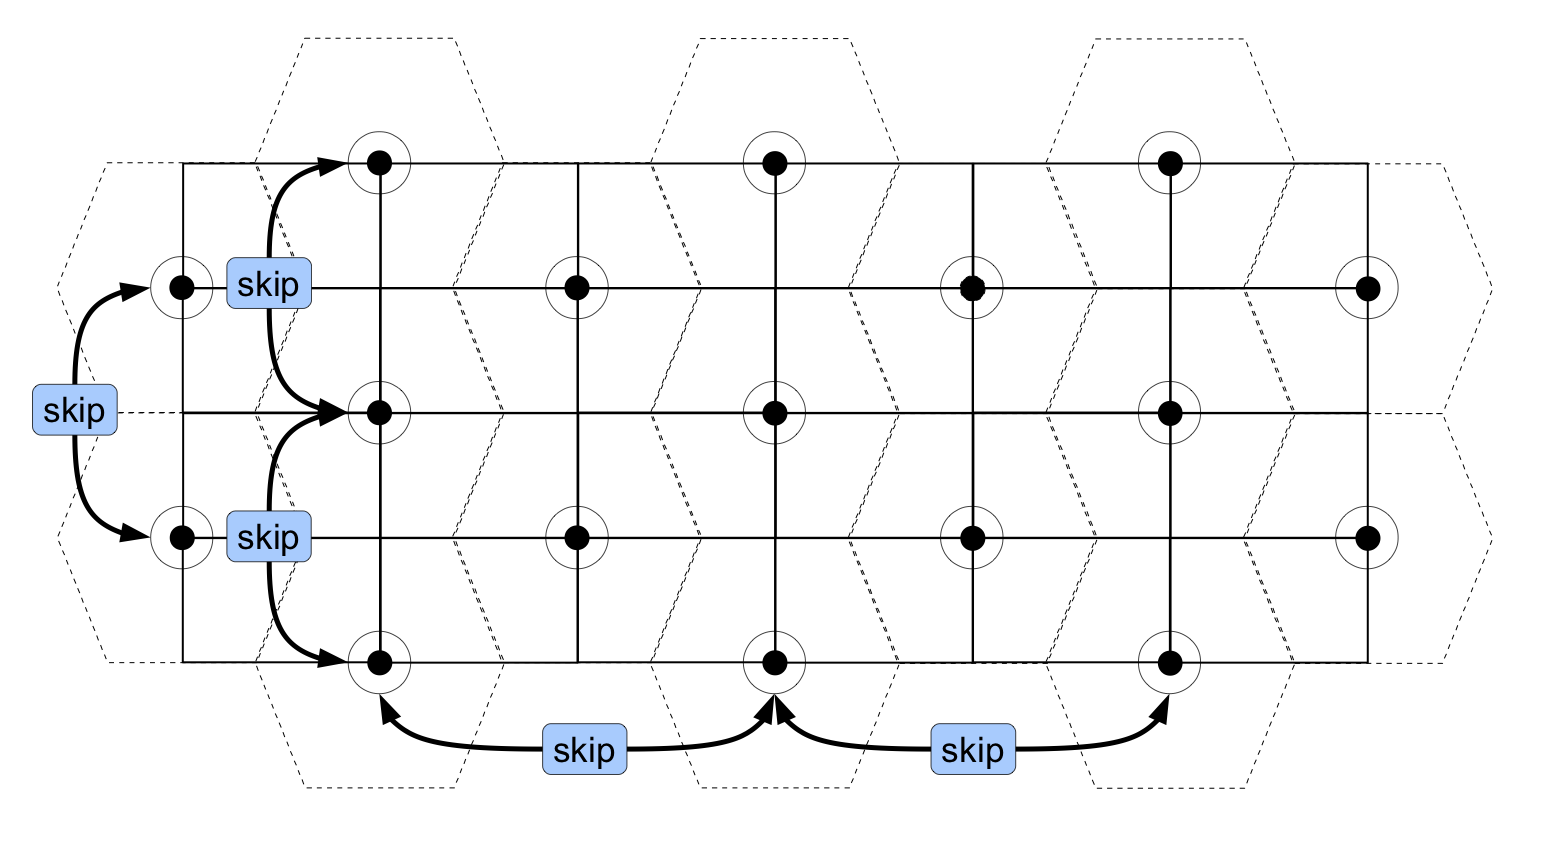
\includegraphics[width=21.46in]{figures/grid2a} 

}

\caption{Selecting alternating intersections of the grid in the x and y directions to spread sampling points evenly}\label{fig:grid2b}
\end{figure}

Note how this process places sampling points at the centres of hexagons
in a hexagonal grid without the need to draw a hexagonal grid.

Make sure that your sample points go right to the edge (or even over the
edge) of the survey area. This helps to ensure that the survey will
sample from the entire survey area.

\newpage

\hypertarget{step-5-select-the-communities-to-sample}{%
\section{Step 5: Select the communities to
sample}\label{step-5-select-the-communities-to-sample}}

\begin{figure}[H]

{\centering 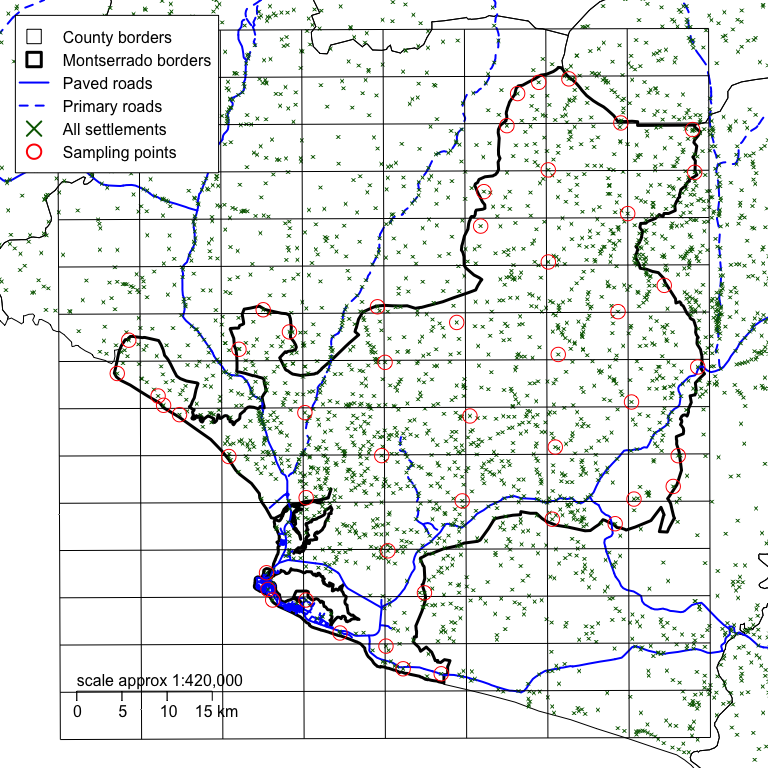
\includegraphics{figures/grid3-1} 

}

\caption{Montserrado county with a rectangular grid defined by d of 6 km and sampling points moved to the nearest communities}\label{fig:grid3}
\end{figure}

\newpage

\begin{figure}[H]

{\centering 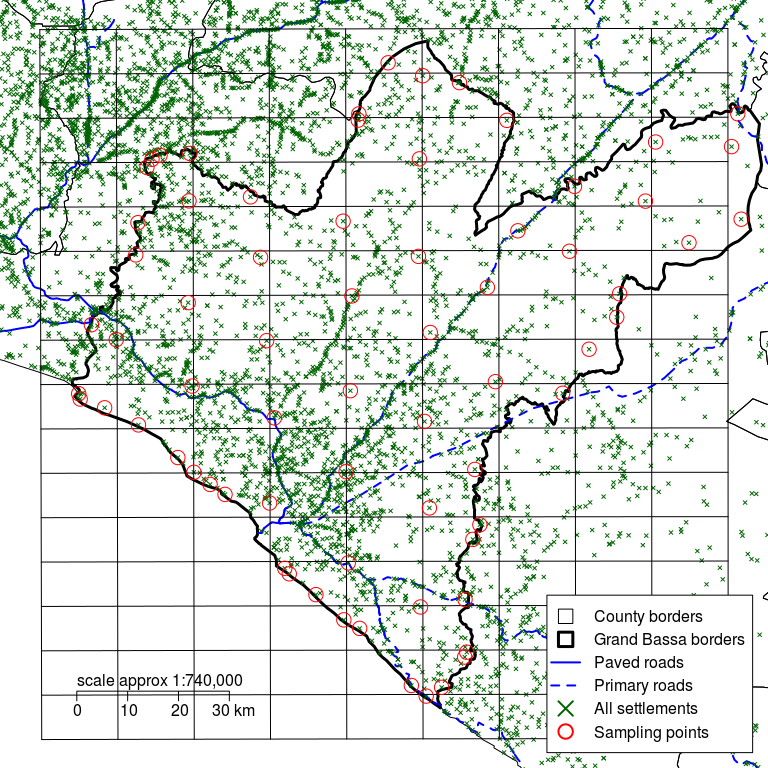
\includegraphics{figures/grid4-1} 

}

\caption{Grand Bassa county with a rectangular grid defined by d of 10 km and sampling points moved to the nearest communities}\label{fig:grid4}
\end{figure}

Select the community (or communities) closest to the sampling points
identified in \textbf{Step 4}.

The position of the sampling point is moved to the position of the
selected community. This is shown in the diagram above.

You may drop sampling points if you find that many sampling points are
clustered closely together.

You may move or add sampling points if you find that there are populated
areas that do not contain sampling points.

The aim is to create a roughly even spread of sampling points over the
entire survey area.

\BeginKnitrBlock{rmdcaution}
The S3M sample is defined using a systematic sampling method. Like any
systematic sampling method, an S3M sample can produce biased estimates
if there is periodic variation in prevalence and / or coverage and the
sampling points tend to coincide with this periodicity. This is
difficult to control for without prior knowledge of the periodic
variation, although simple checks such as ensuring that sampling points
are not all in valleys or all on hilltops, and adjusting the grid
position accordingly, should help to minimise this problem.
\EndKnitrBlock{rmdcaution}

\begin{figure}[H]

{\centering 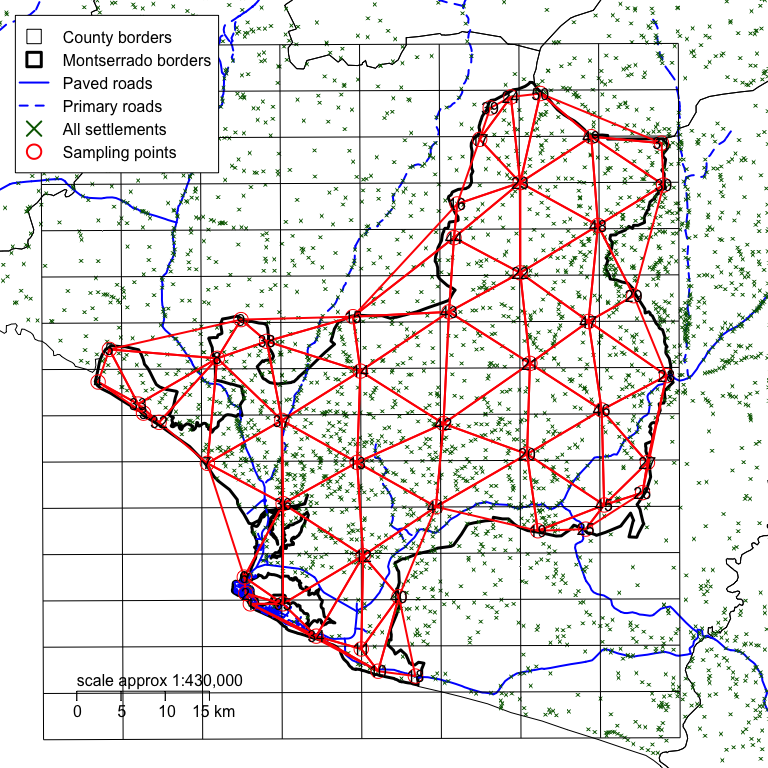
\includegraphics{figures/grid3a-1} 

}

\caption{Montserrado county with a rectangular grid defined by d of 6 km and sampling points moved to the nearest communities showing test triangulation}\label{fig:grid3a}
\end{figure}

\begin{figure}[H]

{\centering 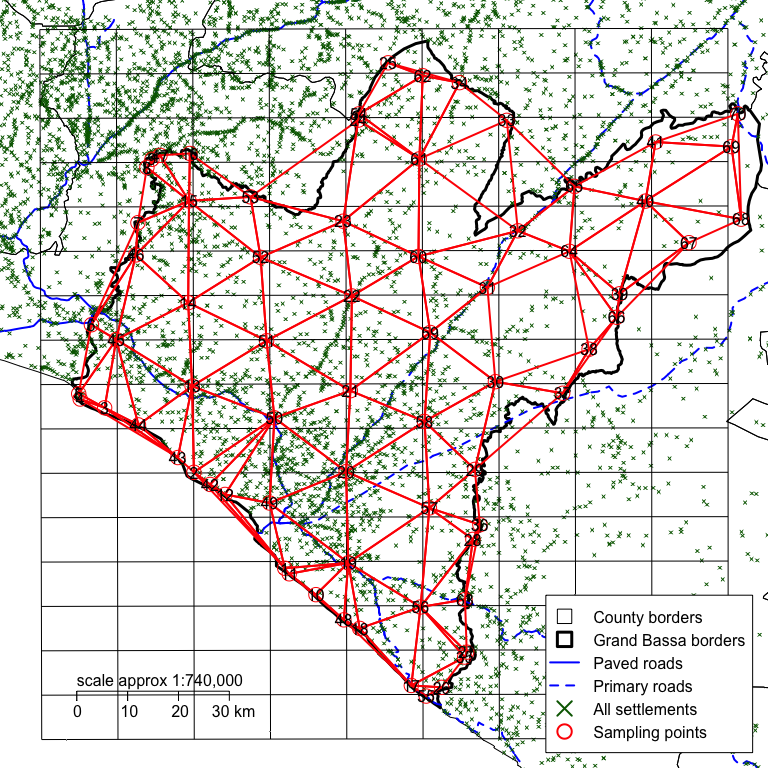
\includegraphics{figures/grid4a-1} 

}

\caption{Grand Bassa county with a rectangular grid defined by d of 10 km and sampling points moved to the nearest communities showing test triangulation}\label{fig:grid4a}
\end{figure}

A good way to check if you have an even spread of sampling points over
the entire survey area is to do a trial \emph{triangulation} of the
selected sampling points. This involves dividing up the survey area into
non-overlapping triangles with a sampling point at each vertex.

There will usually be many ways to divide the survey area into
triangles. The best triangulation is one that results in small
equilateral triangles (i.e.~triangles with all sides of equal length) or
small and nearly equilateral triangles. Avoid long and narrow triangles.
Avoid large triangles.

\begin{figure}[H]

{\centering 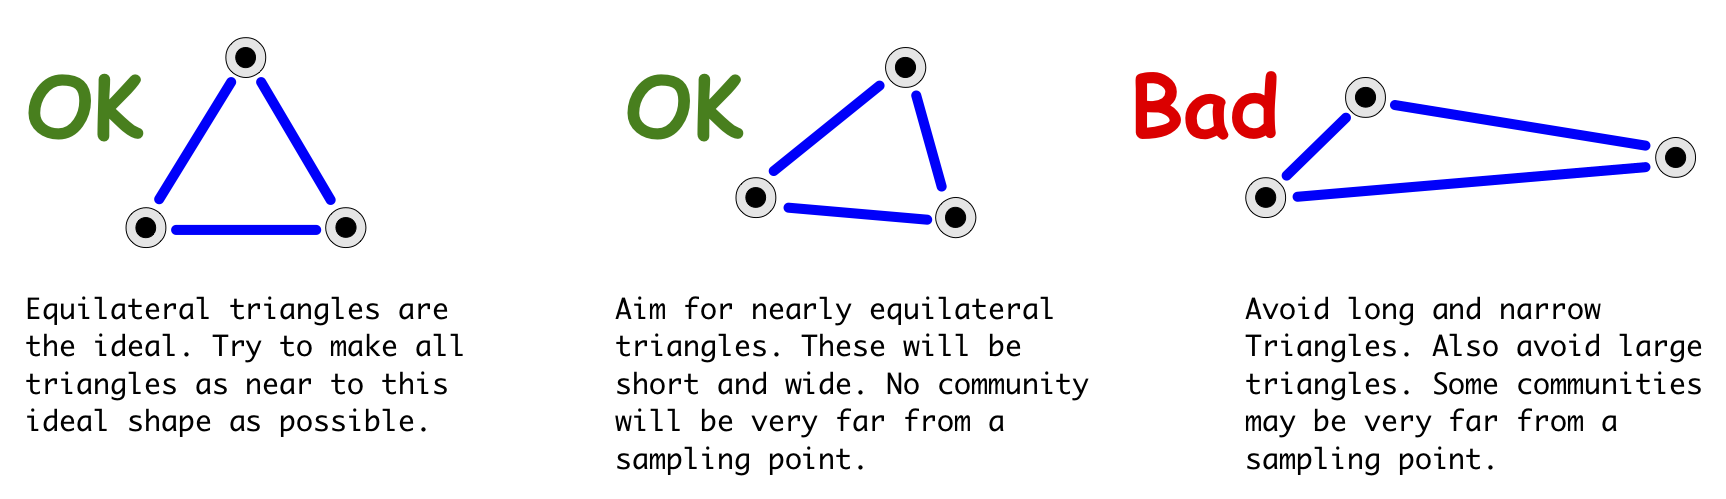
\includegraphics[width=23.97in]{figures/grid3a} 

}

\caption{Selecting alternating intersections of the grid in the x and y directions to spread sampling points evenly}\label{fig:grid3b}
\end{figure}

You can triangulate ``by eye'' or automatically (i.e.~using a computer).
If you use a computer to do this then you should use software that
produces a \emph{Delaunay triangulation}.

You may drop sampling points if you find that many sampling points are
clustered closely together.

You may move or add sampling points if you find that there are populated
areas that do not contain sampling points.

The aim is to create a roughly even spread of sampling points over the
entire survey area.

\newpage

\begin{figure}[H]

{\centering 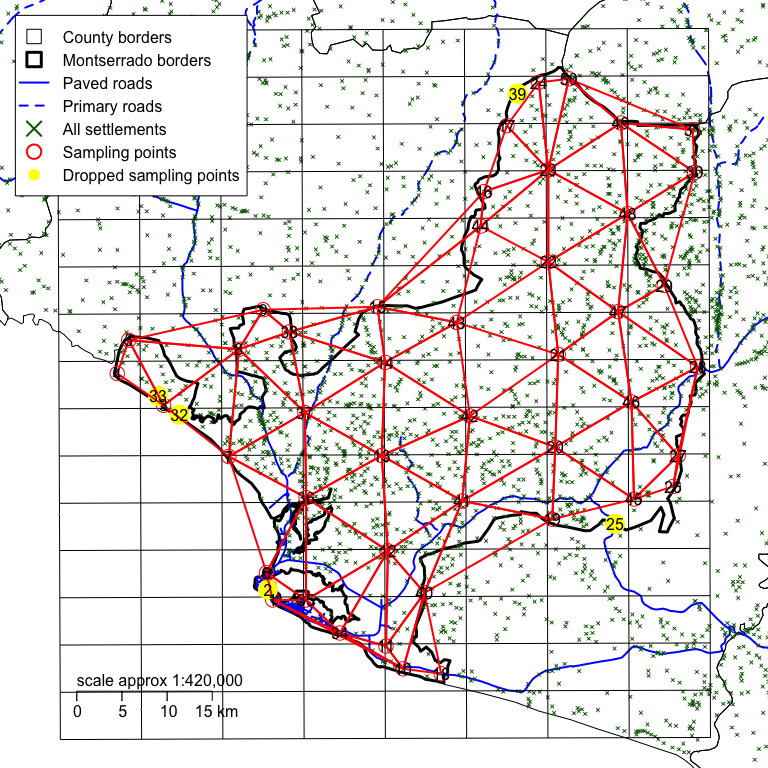
\includegraphics{figures/grid3c-1} 

}

\caption{Montserrado county with a rectangular grid defined by d of 6 km and sampling points moved to the nearest communities showing updated triangulation}\label{fig:grid3c}
\end{figure}

\begin{figure}[H]

{\centering 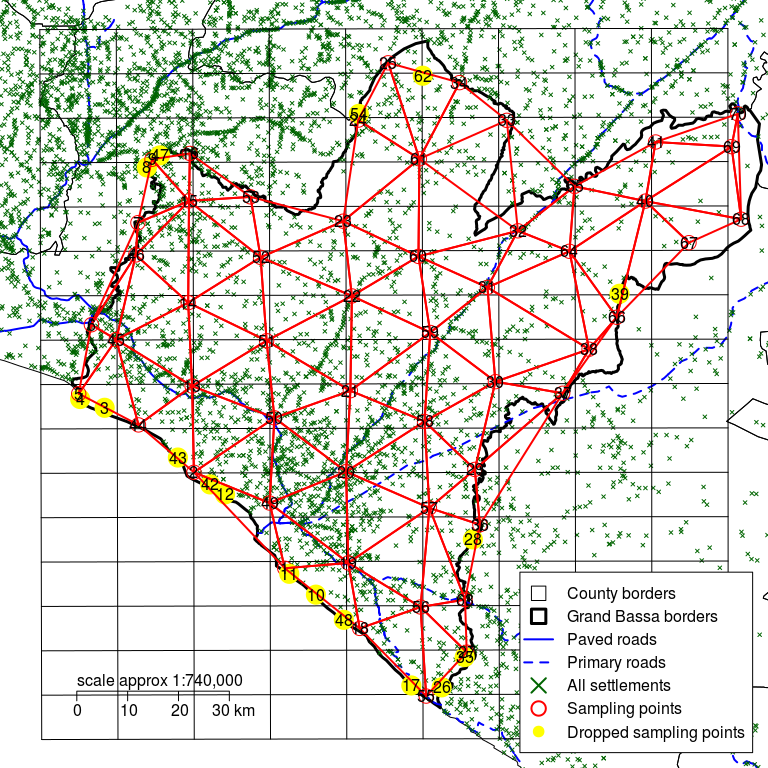
\includegraphics{figures/grid4c-1} 

}

\caption{Grand Bassa county with a rectangular grid defined by d of 10 km and sampling points moved to the nearest communities showing updated triangulation}\label{fig:grid4c}
\end{figure}

Figure \ref{fig:grid3c} above show a trial triangulation for Montserrado
county with only a few long and narrow triangles. Five sampling points
(labelled 2, 25, 32, 33, 39) have been dropped to ensure that there are
few long and narrow triangles.

Figure \ref{fig:grid4c} above show a trial triangulation for Grand Bassa
county with only a few long and narrow triangles. Seventeen sampling
points (labelled 3, 4, 8, 10, 11, 12, 17, 26, 28, 35, 39, 42, 43, 47,
48, 54, 62) have been dropped to ensure that there are a few long and
narrow triangles.

\newpage

\textbf{The sample will, to some extent, be dictated by the distribution
of communities in the survey area. It is usual to find that you have
some large triangles and some long and narrow triangles in your final
triangulation. You should try to keep the number of these ``problem''
triangles to a minimum.}

The process of selecting communities to sample is:

\begin{enumerate}
\def\labelenumi{\arabic{enumi}.}
\item
  Start by defining the sample using the grid based approach outlined
  above.
\item
  Use a trial triangulation. This can be done ``by eye'' or using a
  computer. Check for an even spatial sample:
\end{enumerate}

\begin{itemize}
\item
  Most triangles should be short and wide.
\item
  Very few triangles should be long and narrow.
\item
  The triangles should be of roughly equal size.
\item
  The complete set of triangles should cover all (or almost all) of the
  survey area.
\end{itemize}

\begin{enumerate}
\def\labelenumi{\arabic{enumi}.}
\setcounter{enumi}{2}
\tightlist
\item
  Move or add sampling points to improve the sample (i.e.~to avoid long
  and narrow triangles, to avoid large triangles, to make triangles
  roughly equal in size, and to ensure the sample covers all or almost
  all of the survey area). Triangulate again. Repeat this process until
  you are happy with the sample.
\end{enumerate}

\hypertarget{stage2}{%
\chapter{The second stage sample}\label{stage2}}

\hypertarget{step-10-within-community-sampling}{%
\section{Step 10: Within-community
sampling}\label{step-10-within-community-sampling}}

The sampling process that you use to select a sample from a community
will depend on what the survey is investigating.

If you are investigating multiple indicators which apply to different
groups of individuals then you may find it easier to use different
sampling methods for different indicators. You can think of this as
having different surveys for different indicators sampled from the same
set of communities at the same time. For the Liberia S3M, this is the
approach that will be used. There will be a survey for CMAM coverage, a
survey for children under 60 months, a survey for children under 24
months and a survey for pregnant and lactating women.

For the survey for CMAM coverage, an active and adaptive (snowball)
case-finding method will be used in stage 2 sampling to find all or
nearly all of SAM cases in the stage 1 sample.

For the under 60 months and under 24 months sample, this can be
implemented in a single survey in such a way that a large enough under
60 months children are sampled to provide the minimum sample size needed
for the under 24 months survey.

For the survey for pregnant and lactating women, this can be approached
in a couple of ways. The standard approach to evaluating such indicators
is to sample women with children less than 24 months. The expectation
here is that these women are meant to be lactating given their child's
age. At the same time, they have been recently pregnant (within the last
2 years) such that they will be able to recall their pregnancy
experience and be able to report whether or not they benefitted from
ferrous sulfate-folic acid supplementation during their latest
pregnancy. The more complicated approach is to further subdivide this
sample to lactating women (those with children under 24 months old) to
assess the IYCF counselling coverage and then to find all or nearly all
currently pregnant women to ask them about their ferrous sulfate and
folic acid supplementation status. Either approaches will have their
limitations. The main drawback with the second approach is that the
amount of currently pregnant women at any given time is relatively small
(on average about 4 in a village of about 200 population). So, finding
enough sample of pregnant women will always be a challenge. This is the
main reason why standard surveys such as DHS and MICS use the first
approach but with women with children less than 60 months (longer recall
which is problematic).

The most practical stage 2 sample for the Liberia S3M will be a survey
specific for the CMAM coverage in which a part of the survey team will
apply active and adaptive case finding in about 3-5 villages nearest to
the chosen sampling point in stage 1. This is done so as to get enough
sample of SAM cases for estimation. This CMAM coverage survey will then
be nested within an overarching survey of mothers with children under 60
months to assess all other indicators (of the child and of the mother).
This is the most efficient and robust approach given the indicator set
required.

\hypertarget{analysis}{%
\chapter{Analysis}\label{analysis}}

\bibliography{book.bib}


\end{document}
